% This is samplepaper.tex, a sample chapter demonstrating the LLNCS macro
% package for Springer Computer Science proceedings; Version 2.20 of 2017/10/04
%
\documentclass[runningheads]{llncs}
%
\usepackage{graphicx}
\graphicspath{ {./images} }
% Used for displaying a sample figure. If possible, figure files should be
% included in EPS format.
%
% If you use the hyperref package, please uncomment the following line to
% display URLs in blue roman font according to Springer's eBook style:
% \renewcommand\UrlFont{\color{blue}\rmfamily}

\begin{document}
%
    \title{Web Colaborativa com Braid e CRDTs} 
    % \subtitle{Relatório Final da UC de PIIC}
    %
    %\titlerunning{Abbreviated paper title} If the paper title is too long for
    % the running head, you can set an abbreviated paper title here
    %
    \author{João Oliveira\\Orientação de: Nuno Preguiça}
    %
    \authorrunning{João Oliveira, sobre orientação de Nuno Preguiça}
    % First names are abbreviated in the running head. If there are more than
    % two authors, 'et al.' is used.
    %
    \institute{DI - Faculdade de Ciências e Tecnologia - Universidade Nova de
        Lisboa \email{jfv.oliveira@campus.fct.unl.pt}}
    %
    \maketitle              % typeset the header of the contribution
    %
    \begin{abstract}
        Neste relatório exploramos as aplicações {\itshape web} colaborativas e
        a tecnologia que as suporta. É feita uma reflexão sobre as necessidades
        a nível tecnológico, tais como a falta de {\itshape standardização} e as
        dificuldades associadas. Por fim é exposta uma possível solução a estes
        problemas, através da construção de uma solução de sincronização de
        dados.

        \keywords{colaboração, web}
    \end{abstract}
    
    
    % o que este trabalho trata?
    \section{Introdução}

        Nos dias de hoje, as aplicações {\itshape web} colaborativas são uma
        parte cada vez mais importante da vida de qualquer pessoa. Desde a
        marcação de reuniões num calendário partilhado até à realização das
        próprias reuniões, que cada vez mais se fazem em ambientes online.
        Também estão presentes em ambientes menos formais, como na comunicação,
        através de aplicações de {\itshape chatting} ou redes sociais.

        É evidente a popularidade deste tipo de aplicações. Na realidade, estão
        por todo o lado e englobam muito mais do que redes sociais e calendários
        partilhados. A colaboração deixou de ser um nicho e tornou-se o padrão
        em qualquer tipo de aplicação.

        Neste relatório exploramos a tecnologia que está por detrás das
        aplicações {\itshape web} colaborativas e os seus defeitos.

    \section{Trabalho Relacionado}

        % o que é a web colaborativa? (introdução ao tema)
        \subsection{{\itshape Groupware} e Aplicações {\itshape Web} Colaborativas}

        Uma das primeiras definições de {\itshape software} colaborativo surgiu em
        1991, com a designação de {\itshape groupware} ({\itshape group} +
        {\itshape software}) por Ellis et al.: "Especificamente, definimos
        groupware como: sistemas baseados em computadores que suportam grupos de
        pessoas envolvidas numa tarefa (ou objetivo) e que fornecem uma
        interface para um ambiente partilhado"\cite{groupware-def}. 

        Já nos dias de hoje, com esta área muito mais maturada, o contexto em que o
        {\itshape groupware} se encontra é diferente. Devido ao seu alcance
        demográfico, a {\itshape web} e os dispositivos moveis tornaram-se as
        plataformas primárias para difundir serviços de {\itshape groupware}.
        Como exemplo temos serviços como Google Docs, Trello,
        WhatsApp, Facebook, GitHub e muitos mais. 

        Sob este pretexto, podemos destinguir as atuais aplicações {\itshape
        web} colaborativas de outras aplicações {\itshape web} é o facto de
        existir a noção de um estado partilhado para o qual os utilizadores
        contribuem com um objetivo ou propósito em vista, de forma intencional
        ou não. Por exemplo no caso das redes sociais, o objetivo de um
        utilizador é comentar e trocar impressões, com um ou mais utilizadores,
        sobre um tema. Com esse objetivo em vista o utilizador contribui,
        muitas vezes não intencionalmente, para um registo público
        semi-permanente.

        % porque é que isto é releavante? (apresentação leitor<->tema)
        \subsection{Popularidade das Aplicações {\itshape Web} Colabrativas}

        Mesmo na enorme piscina que são as aplicações {\itshape web}, as
        colaborativas são de longe as mais usadas e que trazem mais pessoas para
        a {\itshape web}.

        Um estudo feito em 2021, aponta para que
        57\%\cite{eurostat-soc-media-usage} da população europeia já tenha usado
        redes sociais. Já nos EUA, os valores apontam para tão alto quanto
        70\%\cite{usa-soc-media-usage}. Fora do mundo ocidental os números
        também não ficam muito a baixo, com a China e a India com
        valores\footnote{É importante notar que o relatório citado usa o número
        de utilizadores bruto, ou seja, não filtra utilizadores falsos ou
        duplicados. Não obstante disso, com estas figuras podemos concluir que
        as redes sociais abrangem largas faixas de populações não ocidentais,
        visto o valor obtido para a India ser o mais baixo da região asiática e
        representar cerca de 1/3 da população.} de 68\% e 34\%,
        respetivamente\cite{digital2022}. 
        

    \section{Estado da Arte}

        % a.k.a: o que é que esta treta toda tem a ver com o trabalho?
        \subsection{Problemas de {\itshape standardização} e o Protolo Braid}

        Para as aplicações {\itshape web} colaborativas é essencial a
        sincronização de dados. Logo, a {\itshape standardização} dos protocolos
        de comunicação que são usados para sincronizar esses mesmos dados é
        importante para a interoperabilidade de sistemas. 

        Atualmente, a falta de um protocolo de sincronização geralmente aceite
        leva a que ao longo do desenho de uma aplicação colaborativa se recorra
        a modelos de comunicação {\itshape ad-hoc}, tal como comunicação por
        eventos\footnote{Por exemplo {\itshape socket.io} ou {\itshape
        web-socket}s} ou técnicas como {\itshape long-polling}. 

        % apresentação do Braid
        O Protoclo Braid surge como resposta a este problema.
            
        Segundo a própria equipa Braid o protocolo Braid é "um conjunto de
        extensões que generalizam o protocolo HTTP de um protocolo de
        transferência de estado para um protocolo de sincronização de estado
        [...] colocando o poder de OT e dos CRDTs na web, melhorando a
        performance de rede e permitindo aplicações web serem nativamente
        P2P, colaborativamente editáveis e {\itshape
        offline-first}"\cite{braid-spec}. 

        No fundo, é um protocolo de sicronização de dados que procura ser
        {\itshape backwards-compatible} e que está em desenvolvimento no
        contexto da IETF.

        \subsection{{\itshape CRDT}s}

        Outro aspeto a considerar é como os dados efetivamente são sincronizados.

        Os "Tipos de dados Replicados sem Conflito", habitualmente denominados
        {\itshape CRDT}s (do inglês {\itshape Conflict Free Replicated Data
        Type}s), são abstrações de tipos de dados desenhadas para permitirem a
        replicação de dados por múltiplos processos com coordenação assíncrona,
        através da troca de mensagens entre as réplicas e de métodos
        determinísticos\cite{CRDTs}.

        Mais especificamente, os {\itshape CRDT}s garantem alta disponibilidade
        no acesso a dados replicados, consistência eventual e tolerância a
        falhas de rede. 
        
        Isto torna a tecnologia dos {\itshape CRDT}s muito atrativa,
        especialmente para um sistema que vise suportar aplicações {\itshape
        web} colaborativas distribuidas disponíveis {\itshape offline}. Há soluções
        que fazem uso desta tecnologia tanto no {\itshape backend}, com bases de
        dados replicadas de alta disponibilidade\footnote{Ver Redis
        (https://redis.com/)}, como no {\itshape frontend} das aplicações, onde
        se vêem certas partes de aplicações a serem replicadas por utilizadores
        através da tecnologia dos {\itshape CRDT}s.

        \subsection{Bibliotecas de {\itshape CRDT}s}

        De maneira a aplicar esta tecnologia ao mundo real, é necessário dotar
        os desenvolvedores de {\itshape software} de ferramentas que lhes
        permitam abstrair-se da complexidade do desenho da parte interna dos
        {\itshape CRDT}s. Para tal, existem inúmeras implementações de {\itshape
        CRDT}s que escondem a complexidade atrás de interfaces bem conhecidas,
        como listas, dicionários, árvores, etc., e interfaces de sincronização,
        estas que variam de implementação para implementação.

        Para o teste da nossa solução iremos usar duas bibliotecas de {\itshape
        CRDT}s que ficam abaixo descritas:

        \subsubsection{Legion -} Framework concebido em 2017 que permite a
        aplicações {\itshape web} replicar nos clientes, e de forma segura,
        dados presentes em servidores. Funciona à base de {\itshape deltas}
        ($\Delta$-CRDT), que representam diferenças entre o estado interno de
        dois {\itshape CRDT}s e permitem otimizar o processo de sincronização.

        \subsubsection{Automerge -} Biblioteca para sincronização de dados entre
        dispositivos móveis. Usa os seus próprios {\itshape CRDT}s para oferecer
        um modelo de dados de tipo {\itshape JSON}.

    \section{TejoSynchronizer}

        O {\itshape TejoSynchronizer} é um framework que procura facilitar o
        trabalho do desenvolvedor de aplicações {\itshape web} colaborativas, através de uma interface que
        {\itshape standardiza} a interação com soluções de sincronização
        específicas, como o Legion ou o Automerge.
        
        Nomeadamente, esta solução especifica três componentes:

        \begin{itemize}
            \item \textbf{Sincronizador}: Componente associada à solução de
            sincronização. Implementa um protocolo de sincronização e interage
            com um ou mais mensageiros.
            \item \textbf{Mensageiro}: Permite a troca de mensagens entre
            sincronizadores. 
            \item \textbf{\itshape Parser}: Faz a tradução de mensagens entre
            formatos. Serve, por exemplo, para converter mensagens de um
            Sincronizador para mensagens que podem ser enviadas pelo Mensageiro.
        \end{itemize}
        
        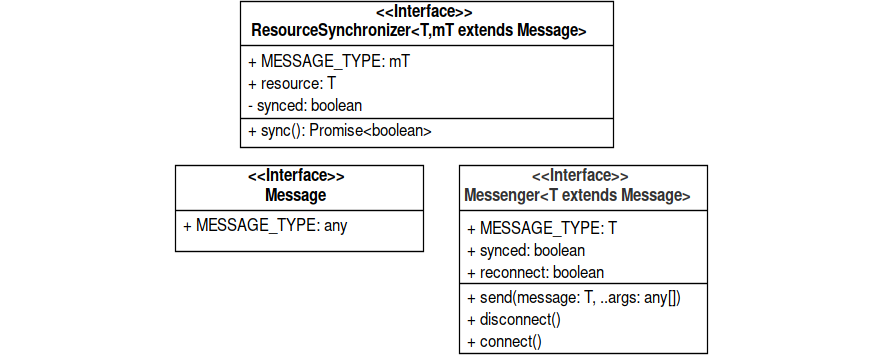
\includegraphics[width=\textwidth]{Interfaces.png}

        Um aspeto importante é o facto de tanto o Sincronizador como o
        Mensageiro são emissores de eventos.

        \paragraph{Sample Heading (Fourth Level)}
        The contribution should contain no more than four levels of headings.
        Table~\ref{tab1} gives a summary of all heading levels.

        \begin{table}
        \caption{Table captions should be placed above the tables.}\label{tab1}
        \begin{tabular}{|l|l|l|}
        \hline
        Heading level &  Example & Font size and style\\
        \hline
        Title (centered) &  {\Large\bfseries Lecture Notes} & 14 point, bold\\
        1st-level heading &  {\large\bfseries 1 Introduction} & 12 point, bold\\
        2nd-level heading & {\bfseries 2.1 Printing Area} & 10 point, bold\\
        3rd-level heading & {\bfseries Run-in Heading in Bold.} Text follows &
        10 point, bold\\
        4th-level heading & {\itshape Lowest Level Heading.} Text follows & 10
        point, italic\\
        \hline
        \end{tabular}
        \end{table}


        \noindent Displayed equations are centered and set on a separate line.F
        \begin{equation}
        x + y = z
        \end{equation}
        Please try to avoid rasterized images for line-art diagrams and schemas.
        Whenever possible, use vector graphics instead (see Fig.~\ref{fig1}).

        %\begin{figure} 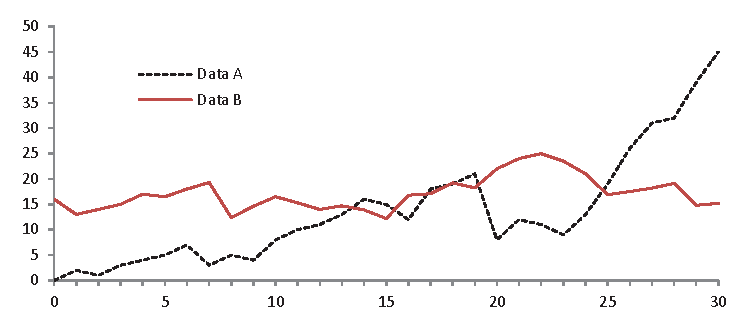
\includegraphics[width=\textwidth]{fig1.eps} \caption{A
        %figure caption is always placed below the illustration. Please note
        %that short captions are centered, while long ones are justified by the
        %macro package automatically.} \label{fig1} \end{figure}

        \begin{theorem}
        This is a sample theorem. The run-in heading is set in bold, while the
        following text appears in italics. Definitions, lemmas, propositions,
        and corollaries are styled the same way.
        \end{theorem}
        %
        % the environments 'definition', 'lemma', 'proposition', 'corollary',
        % 'remark', and 'example' are defined in the LLNCS documentclass as
        % well.
        %
        \begin{proof}
        Proofs, examples, and remarks have the initial word in italics, while
        the following text appears in normal font.
        \end{proof}
        For citations of references, we prefer the use of square brackets and
        consecutive numbers. Citations using labels or the author/year
        convention are also acceptable. The following bibliography provides a
        sample reference list with entries for journal
        articles~\cite{ref_article1}, an LNCS chapter~\cite{ref_lncs1}, a
        book~\cite{ref_book1}, proceedings without editors~\cite{ref_proc1}, and
        a homepage~\cite{ref_url1}. Multiple citations are grouped
        \cite{ref_article1,ref_lncs1,ref_book1},
        \cite{ref_article1,ref_book1,ref_proc1,ref_url1}.
    %
    % ---- Bibliography ----
    %
    % BibTeX users should specify bibliography style 'splncs04'. References will
    % then be sorted and formatted in the correct style.
    %
    % \bibliographystyle{splncs04} \bibliography{mybibliography}
    %

    \bibliographystyle{splncs04}
    \bibliography{refs}

    %\begin{thebibliography}{3}

    %\bibitem{CRDTs} Shapiro, M., Preguiça, N., Baquero, C., Zawirski, M.:
    %Conflict-free replicated data types. In 13th international conference on
    %Stabilization, safety, and security of distributed systems (SSS'11), pp.
    %386–400 Springer-Verlag, Berlin, Heidelberg. 

    %\bibitem{groupware-def}

    %\bibitem{braid-spec} It is inappropriate to use Internet-Drafts as
    %reference material or to cite them other than as "work in progress."

    %\bibitem{collab-def} Marinez-Moyano, I. J. Exploring the Dynamics of
    %Collaboration in Interorganizational Settings, Ch. 4, p. 83, in Schuman
    %(Editor). Jossey-bass, 2006. ISBN 0-7879-8116-8.

    %\bibitem{digital2022}

    %\bibitem{eurostat-soc-media-usage}

    %\bibitem{usa-soc-media-usage}

    %\end{thebibliography}
\end{document}
